\documentclass{beamer}\usepackage[]{graphicx}\usepackage[]{color}
%% maxwidth is the original width if it is less than linewidth
%% otherwise use linewidth (to make sure the graphics do not exceed the margin)
\makeatletter
\def\maxwidth{ %
  \ifdim\Gin@nat@width>\linewidth
    \linewidth
  \else
    \Gin@nat@width
  \fi
}
\makeatother

\definecolor{fgcolor}{rgb}{0.345, 0.345, 0.345}
\newcommand{\hlnum}[1]{\textcolor[rgb]{0.686,0.059,0.569}{#1}}%
\newcommand{\hlstr}[1]{\textcolor[rgb]{0.192,0.494,0.8}{#1}}%
\newcommand{\hlcom}[1]{\textcolor[rgb]{0.678,0.584,0.686}{\textit{#1}}}%
\newcommand{\hlopt}[1]{\textcolor[rgb]{0,0,0}{#1}}%
\newcommand{\hlstd}[1]{\textcolor[rgb]{0.345,0.345,0.345}{#1}}%
\newcommand{\hlkwa}[1]{\textcolor[rgb]{0.161,0.373,0.58}{\textbf{#1}}}%
\newcommand{\hlkwb}[1]{\textcolor[rgb]{0.69,0.353,0.396}{#1}}%
\newcommand{\hlkwc}[1]{\textcolor[rgb]{0.333,0.667,0.333}{#1}}%
\newcommand{\hlkwd}[1]{\textcolor[rgb]{0.737,0.353,0.396}{\textbf{#1}}}%

\usepackage{framed}
\makeatletter
\newenvironment{kframe}{%
 \def\at@end@of@kframe{}%
 \ifinner\ifhmode%
  \def\at@end@of@kframe{\end{minipage}}%
  \begin{minipage}{\columnwidth}%
 \fi\fi%
 \def\FrameCommand##1{\hskip\@totalleftmargin \hskip-\fboxsep
 \colorbox{shadecolor}{##1}\hskip-\fboxsep
     % There is no \\@totalrightmargin, so:
     \hskip-\linewidth \hskip-\@totalleftmargin \hskip\columnwidth}%
 \MakeFramed {\advance\hsize-\width
   \@totalleftmargin\z@ \linewidth\hsize
   \@setminipage}}%
 {\par\unskip\endMakeFramed%
 \at@end@of@kframe}
\makeatother

\definecolor{shadecolor}{rgb}{.97, .97, .97}
\definecolor{messagecolor}{rgb}{0, 0, 0}
\definecolor{warningcolor}{rgb}{1, 0, 1}
\definecolor{errorcolor}{rgb}{1, 0, 0}
\newenvironment{knitrout}{}{} % an empty environment to be redefined in TeX

\usepackage{alltt}
\usepackage{xcolor}
\usepackage{graphicx}
\usepackage{tikz}
\usetikzlibrary{shapes.geometric, arrows}
\usepackage{verbatim}
\definecolor{UAred}{RGB}{204,0,51}
\definecolor{UAblue}{RGB}{0,51,102}

\useoutertheme{infolines}%makes informative footer
\usetheme{Pittsburgh}
\setbeamercolor{structure}{fg=UAblue}
\setbeamercolor{normal text}{fg=black}
\setbeamercolor{upper separation line head}{bg=UAred}
\AtBeginSection{\frame{\sectionpage}}%make section title pages
\AtBeginSubsection{\frame{\subsectionpage}}

\setbeamertemplate{headline}
{
  \leavevmode
  \hbox{
  \begin{beamercolorbox}[wd=.5\paperwidth,ht=6ex,dp=2ex,left,rightskip=1em]{section in head/foot}%
    \usebeamerfont{subsection in head/foot}\hspace*{2ex}\insertshorttitle
  \end{beamercolorbox}
  \begin{beamercolorbox}[wd=.25\paperwidth,ht=6ex,dp=1ex,left,leftskip=1em]{subsection in head/foot}%
    \usebeamerfont{section in head/foot}\insertsectionhead\hspace*{2ex}
  \end{beamercolorbox}
  \begin{beamercolorbox}[wd=.25\paperwidth,ht=6ex,dp=1ex,right,leftskip=1em]{subsection in head/foot}%
    
\includegraphics[scale=.15]{./Figures/UA_CPH_RGB_Primary.png}
  \end{beamercolorbox}}
  \begin{beamercolorbox}[colsep=1.5pt,ht=.75ex]{upper separation line head}
  \end{beamercolorbox}
  \vskip0pt%
}

\setbeamertemplate{footline}
{
  \leavevmode
  \hbox{%

\begin{beamercolorbox}[wd=.70\paperwidth,ht=4.25ex,dp=4ex,left,leftskip=2ex]{title in head/foot}%
    \usebeamerfont{title in head/foot}\insertshorttitle{} - \insertshortauthor
\end{beamercolorbox}%
\begin{beamercolorbox}[wd=.20\paperwidth,ht=4.25ex,dp=4ex,center]{date in head/foot}%
    \usebeamerfont{date in head/foot}\insertshortdate{}
\end{beamercolorbox}%
\begin{beamercolorbox}[wd=.10\paperwidth,ht=4.25ex,dp=4ex,right,rightskip=2ex]{date in head/foot}%
    \insertframenumber{} / \inserttotalframenumber
  \end{beamercolorbox}}%
\vskip0pt%
}

\setbeamertemplate{frametitle}{%place the title in the center
\vspace*{4mm}\hspace*{-2mm}\insertframetitle
}

\setbeamertemplate{navigation symbols}{}%remove Navigation Symbols
%start entering presentation specific stuff below here...
%start entering presentation specific stuff below here...%%%%%%%%%%%%%%%%%%%%%%%%%%%%%%%%%%%%%%%%%%%%%%%
\title[Correlation in Relative Data]{Problems with Correlations in Relative Data and a Proposed Alternative}
\author[Dominic LaRoche]{Dominic LaRoche}
\IfFileExists{upquote.sty}{\usepackage{upquote}}{}
\begin{document}

\maketitle

\begin{frame}{The Papers}
\begin{center}
\large{\textbf{Proportionality: A Valid Alternative to Correlation for Relative Data}}\\
\small{David Lovell, Vera Pawlowsky-Glahn, Juan José Egozcue, Samuel Marguerat, and Jürg Bähler\\
PLoS Computational Biology 11(3) (2015)}\\

\bigskip
\large{\textbf{Proportions, Percentages, PPM: Do the Molecular Biosciences Treat Compositional Data Right?}}\\
\small{Lovell DR, Muller W, Taylor JM, Zwart AB, Helliwell CA\\
Compositional data analysis: Theory and applications p193-207 (2011)}
\end{center}
\end{frame}


\section{Introduction to the Problem}

\begin{frame}{What is Relative Data? --Also called ``Compositional Data"}
\begin{itemize}
\item Compositional data are vectors of non-negative components showing the \emph{relative} weight or importance of a set of \emph{parts in a total}
\bigskip
\item The total sum of a compositional vector is considered irrelevant, or an artifact of the sampling procedure.
\bigskip
\item No individual component can be interpreted isolated from the other. A composition carries no absolute information on increment/decrement of mass.
\end{itemize}
\end{frame}

\begin{frame}{Is \emph{my} data relative??}
Relative data arises naturally in many biological measurements:
\begin{itemize}
\item Is your sample oa fixed size?
  \begin{itemize}
  \item 1 gram of tissue
  \item 1 $\mu$g of total RNA
  \item 1 $\mu$g of metagenomic DNA
  \item 1 mL of blood, etc.
  \end{itemize}
\pause
\smallskip
\item Is your data a constrained count?
  \begin{itemize}
  \item How many total reads can your favorite platform handle?
  \item Counts of codons or bases in a fixed length of DNA
  \end{itemize}
\pause
\smallskip
\item Is your data based on proportions?
  \begin{itemize}
  \item Different k-mers in genomes
  \item GO terms in samples
  \item different reads in NGS sequencing runs
  \end{itemize}
\end{itemize}
\pause
\bigskip
\textbf{Then your data might be relative!}
\end{frame}

\begin{frame}{Should I \emph{care} if my data is relative??}
\pause
\textbf{Yes}\\
\bigskip
\pause
Long answer:  It depends...\\
\bigskip
In certain cases it doesn't matter much but in others it matters a lot.
\end{frame}

\begin{frame}{The `Omics Imp'}
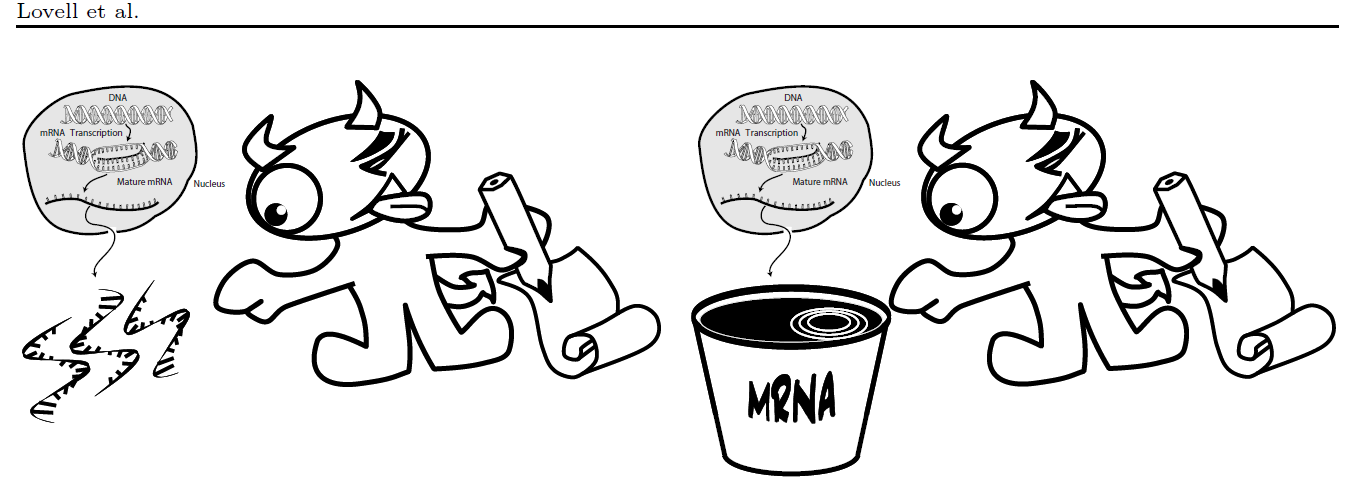
\includegraphics[scale=.4]{./Figures/OmicsImp}\\
\begin{itemize}
\item On the left the imp tallies sequences as they are produced in a fixed time period
\item On the right the imp counts the sequences in some fixed size bucket
  \begin{itemize}
  \item Data on the right are parts of a total
  \end{itemize}
\end{itemize}
\end{frame}

\begin{frame}{Relative data can be misleading}
Example 1.\\
\begin{center}
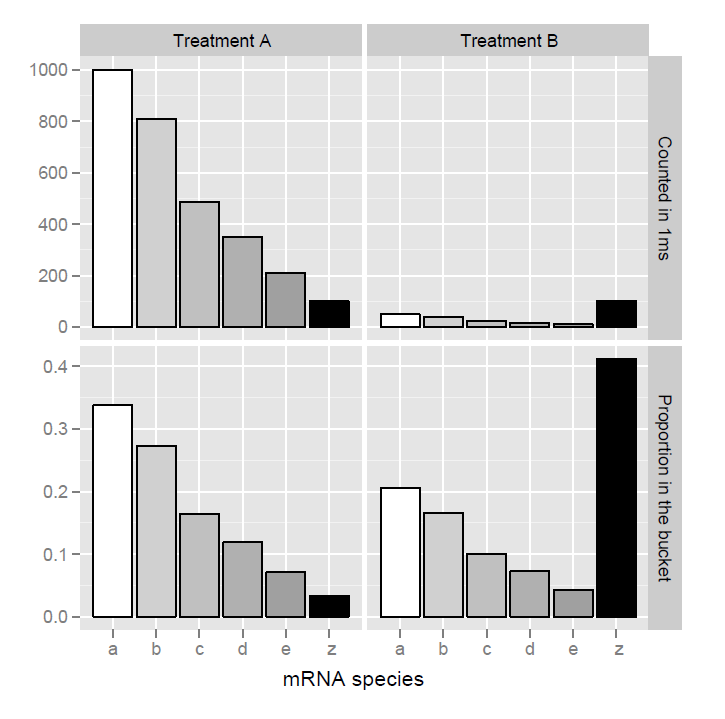
\includegraphics[scale=.4]{./Figures/Zconstant}
\end{center}
\end{frame}

\begin{frame}{Relative data can be misleading}
Example 2.\\
\begin{center}
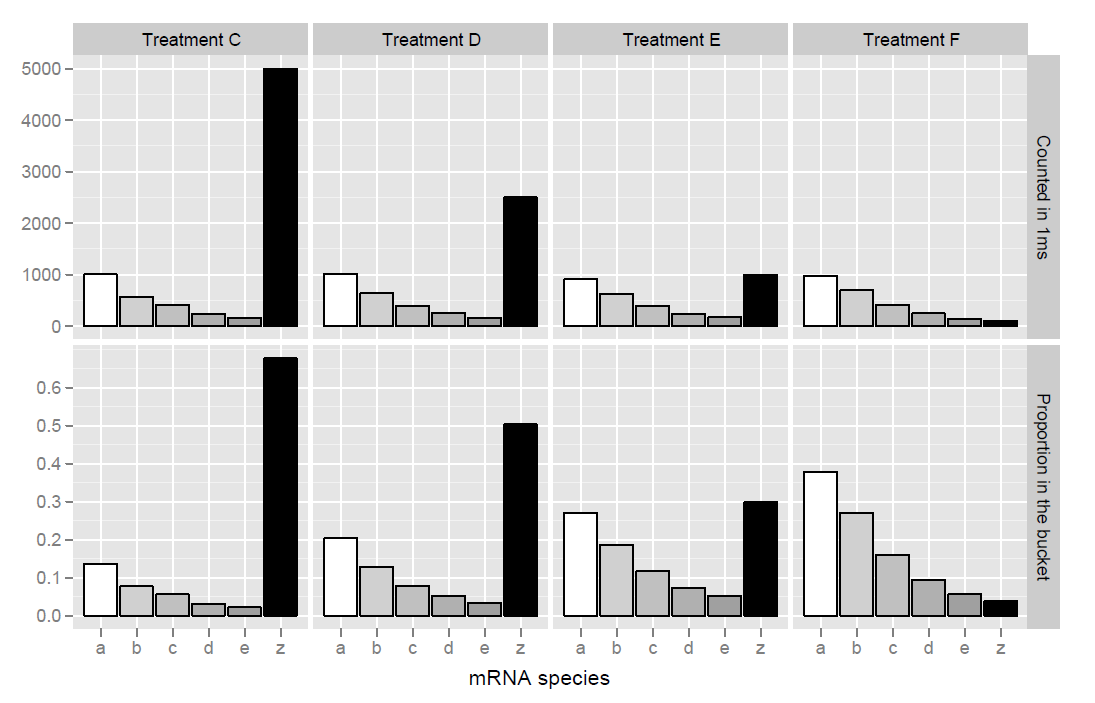
\includegraphics[scale=.4]{./Figures/AEconstant}
\end{center}
\end{frame}

\begin{frame}{When is relative data likely to be misleading?}
Take a 3 component example: $Total = c_1 + c_2 + c_3$
\pause
\bigskip
\begin{itemize}
\item $c_1, c_2 \gg c_3$
  \begin{itemize}
  \item As $c_1 \uparrow$ then $c_2 \downarrow$
  \item Correlation is attenuated
  \end{itemize}
\pause
\bigskip
\item $c_3 \gg c_1, c_2$
  \begin{itemize}
  \item Here $var\left(c_3\right)$ dominates the composition
  \item Correlation is biased high as $var\left(c_3\right) \uparrow$
  \end{itemize}
\end{itemize}
\end{frame}

\begin{frame}{Correlations on Relative Data}
Yes, I am going to show a slide show during a slide show.\\
\bigskip
\href{http://www.slideshare.net/AustralianBioinformatics/dont-correlate-proportions}{David Lovell scaring you about correlating proportions}
\end{frame}


\begin{frame}{When can I mostly ignore the relative nature of my data?}
\end{frame}
\end{document}
